\begin{figure}[H]
  \centering
  \begin{subfigure}[b]{0.2\textwidth}
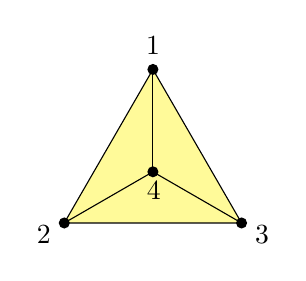
\begin{tikzpicture}
    % Define the length of the side of the triangle
    \def\side{1.3}
    % Draw the equilateral triangle centered at (0,0)
    \filldraw[fill=yellow!40] (90: \side) -- (210: \side) -- (330: \side) -- cycle;
    % Connect the center with all three vertices
    \draw (0,0) -- (90: \side);
    \draw (0,0) -- (210: \side);
    \draw (0,0) -- (330: \side);

    % Label the vertices and the center
    \node at (90: \side + 0.3) {1};
    \node at (210: \side + 0.3) {2};
    \node at (330: \side + 0.3) {3};
    \node at (-0.2,0) [below right] {4}; % You can adjust the position of this label

    % Optionally, mark the center
    \fill (90: \side) circle (2pt);  % Vertex 1
    \fill (210: \side) circle (2pt); % Vertex 2
    \fill (330: \side) circle (2pt); % Vertex 3
    \fill (0,0) circle (2pt);        % Center 4
\end{tikzpicture}
\caption{$\LL$}%
\end{subfigure}%
\quad
\begin{subfigure}[b]{0.2\textwidth}
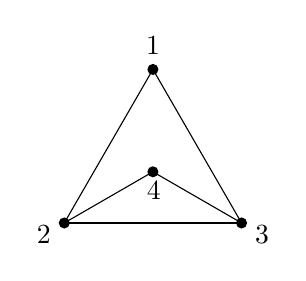
\begin{tikzpicture}
    % Define the length of the side of the triangle
    \def\side{1.3}

    % Fill the equilateral triangle centered at (0,0)
    % Use \fill instead of \filldraw to avoid drawing the edge between 1 and 2
    %\fill[fill=yellow!40] (90: \side) -- (210: \side) -- (330: \side) -- cycle;
    
    % Draw the edges between the other two pairs of vertices
    \draw (210: \side) -- (330: \side); % Edge between vertices 2 and 3
    \draw (330: \side) -- (90: \side);  % Edge between vertices 3 and 1
    \draw (90: \side) -- (210: \side);

    % Connect the center with all three vertices
    %\draw (0,0) -- (90: \side);
    \draw (0,0) -- (210: \side);
    \draw (0,0) -- (330: \side);

    % Fill the vertices with yellow circles (2pt)
    \fill (90: \side) circle (2pt);  % Vertex 1
    \fill (210: \side) circle (2pt); % Vertex 2
    \fill (330: \side) circle (2pt); % Vertex 3
    \fill (0,0) circle (2pt);        % Center 4

    % Label the vertices and the center
    \node at (90: \side + 0.3) {1};
    \node at (210: \side + 0.3) {2};
    \node at (330: \side + 0.3) {3};
    \node at (-0.2,0) [below right] {4};
\end{tikzpicture}
\caption{$\KK$.}
\end{subfigure}
\caption{The simplicial complexes $\KK\hookrightarrow \LL$ associated with Example \ref{ex_1}.}%
\label{fig_simplicial_cmplexes}
\end{figure}